\documentclass[14pt]{beamer}
\usepackage[T2A]{fontenc}
\usepackage[utf8]{inputenc}
\usepackage[english,russian]{babel}
\usepackage{amssymb,amsfonts,amsmath,mathtext}
\usepackage{cite,enumerate,float,indentfirst}
\usepackage{longtable}  
\graphicspath{{../assets/}{images/}} 

\usetheme{Pittsburgh}
\usecolortheme{whale}

\setbeamercolor{footline}{fg=blue}
\setbeamertemplate{footline}{
  \leavevmode%
  \hbox{%
  \begin{beamercolorbox}[wd=.333333\paperwidth,ht=2.25ex,dp=1ex,center]{}%
    А. С. Тощев, К(П)ФУ
  \end{beamercolorbox}%
  \begin{beamercolorbox}[wd=.333333\paperwidth,ht=2.25ex,dp=1ex,center]{}%
    Казань, 2015
  \end{beamercolorbox}%
  \begin{beamercolorbox}[wd=.333333\paperwidth,ht=2.25ex,dp=1ex,right]{}%
  Стр. \insertframenumber{} из \inserttotalframenumber \hspace*{2ex}
  \end{beamercolorbox}}%
  \vskip0pt%
}

\newcommand{\itemi}{\item[\checkmark]}

\title{\small{Интеллектуальная система повышения эффективности IT службы предприятия}}
\author{\small{%
\emph{Выступающий:} А.C. Тощев\\%
\emph{Руководитель:} проф., д.ф.-м.н. А.М.Елизаров}\\%
\vspace{30pt}%
Казанский (Приволжский)\\
федеральный университет%
\vspace{20pt}%
}
\date{\small{Казань, 2015}}

\begin{document}

\maketitle

\begin{frame}
\frametitle{Цели и задачи}
\begin{itemize}
  \item \textbf{Предмет исследования} процесс регистрации и устранения проблемных ситуаций, возникающих в IT-инфраструктуре предприятия 
  \item \textbf{Цель исследования}  разработка интеллектуальной системы повышения эффективности деятельности IT-службы предприятия
  \item \textbf{Актуальность} определяется потребностью предприятий IT-отрасли в интеллектуальных системах, повышающих эффективность служб, поддерживающих IT-инфраструктуру этих предприятий
\end{itemize}
\end{frame}

\begin{frame}
\frametitle{Цели и задачи}
\begin{itemize}
    \item \textbf{Область исследования} разработка методов и алгоритмов решения задач системного анализа, оптимизации, управления, принятия решений и обработки информации в IT-отрасли %сузить
\end{itemize}
\end{frame}

\begin{frame}
\frametitle{Структура диссертации}
\begin{enumerate}
  \item \textbf{Глава 1. Обзор существуюших решений}
  \begin{itemize}
    \item Сравнительный анализ систем
    \item Необходимые критерии системы
    \item Сравнительный анализ средств NLP
    \item Выводы
  \end{itemize}
  \item \textbf{Глава 2. Создание модели системы}
  \begin{itemize}
    \item Модель Menta 0.1
    \item Модель Menta 0.3
    \item Модель TU 1.0
    \item Выводы
  \end{itemize}
  \item \textbf{Глава 3. Реализация модели системы}
  \begin{itemize}
    \item Архитектура системы
    \item Модель данных TU Knowledge
    \item Прототип системы
    \item Выводы
  \end{itemize}
 \end{enumerate}
\end{frame}

\begin{frame}
\frametitle{Структура диссертации}
\begin{enumerate}
 \item \textbf{Глава 4. Экспериментальные исследования}
  \begin{itemize}
    \item Экспериментальные данные
    \item Оценка эффективности
    \item Результаты экспериментов
  \end{itemize}

\end{enumerate}
\end{frame}

\begin{frame}
\frametitle{Анализ и определение области исследования}
\begin{figure} [h] 
  \center
  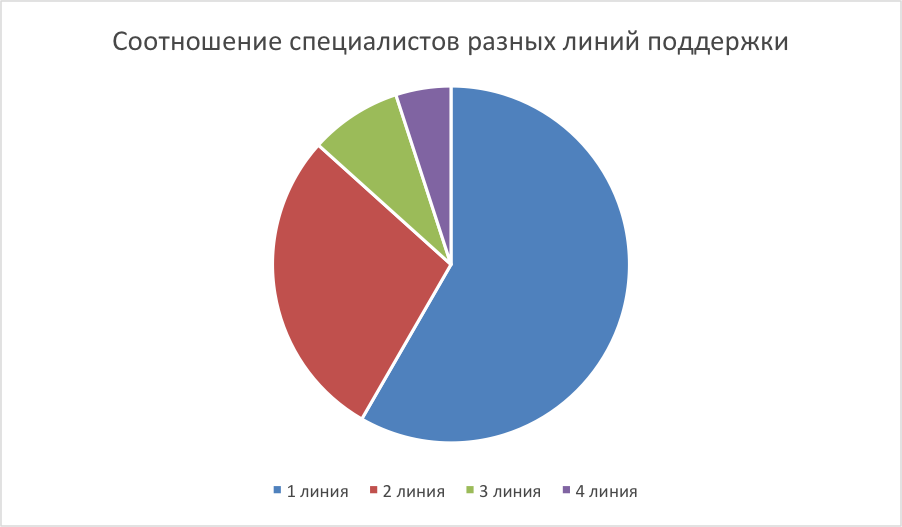
\includegraphics [scale=0.7] {ITSMTeamComposition}
  \label{img:ITSMTeamComposition}  
\end{figure}

\end{frame}

\begin{frame}
\frametitle{Категории инцидентов}
\begin{figure} [h] 
  \center
  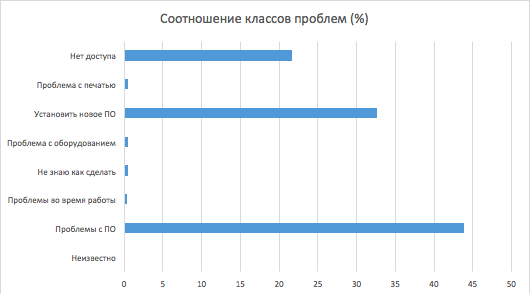
\includegraphics [scale=0.6] {EngineerTasks}
  \label{img:EngineerTasks}  
\end{figure}
\end{frame}


\begin{frame}
\frametitle{Глава 2. Анализ текущих решений}
\begin{table}
	
\small
\begin{tabular} {|p{5cm}|p{1cm}|p{1cm}|p{1cm}|p{1cm}|}

\hline
\textbf{Пункт} & HP Open View & Service NOW & IBM Watson & TU\\
\hline
   Мониторинг & Да & Да & Да & Нет \\
   \hline
   Регистрация инцидентов & Да & Да & Да & Нет\\
   \hline
   Управление системами & Да & Нет & Нет & Нет \\
   \hline 
   Создание цепи обработки & Да & Да & Нет & Да \\
   \hline 
   Запросы на естественном языке & Нет & Нет & Да & Да\\
   \hline 
   Поиск решений & Нет & Нет & Да & Да\\
   \hline 
   Применение решений & Нет & Нет & Нет & Да \\
   \hline
   Обучение & Нет & Нет & Нет & Да \\
   \hline
   Логические рассуждения & Нет & Нет & Нет & Да \\
   \hline
  
\end{tabular}
\end{table}
\end{frame}

\begin{frame}
\frametitle{Глава 3. Теоретическое обоснование}
	\begin{itemize}
		\item  Модель мышления 6-ти Марвина Мински.
	\end{itemize}
\begin{figure} [h] 
  \center
  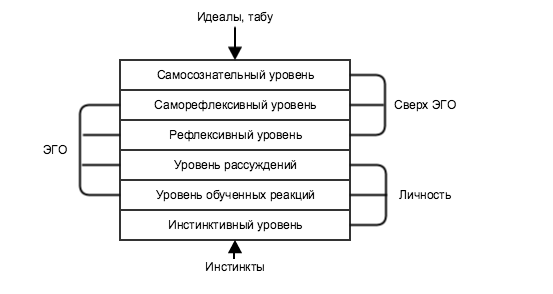
\includegraphics [scale=0.6] {thinkinglevels}
  \caption{Иллюстрация концепции Уровней мышления} 
  \label{img:thinkinglevels}  
\end{figure}
\end{frame}


\begin{frame}
\frametitle{Критик-Селектор-Образ мышления}
\begin{figure} [h] 
  \center
  \includegraphics [scale=0.6] {CSW_EX}
  \caption{Критик-Селектор-Путь мышления в разрезе ресурсов} 
  \label{img:csw_ex}  
\end{figure}
\end{frame}

\begin{frame}
\frametitle{Глава 4. Результаты работы}
\begin{figure} [h] 
  \center
  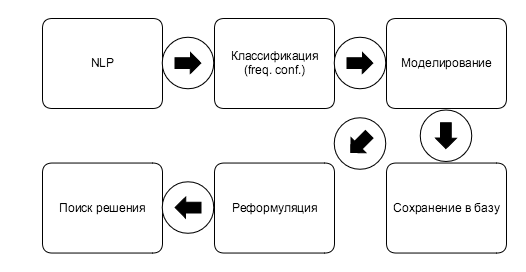
\includegraphics [scale=0.6] {workflow}
  \caption{} 
  \label{img:workflow}  
\end{figure}
\end{frame}

\begin{frame}
\frametitle{Результаты работы}
\begin{table}
	
\small
\begin{tabular} {|p{8cm}|p{1cm}|p{1cm}|}

\hline
\textbf{Запрос} & TSS1 & TU \\
\hline
  Tense is kind of concept. & 15000 & 385 \\
  
  \hline
  Please install Firefox.  & 9000 & 859 \\
  \hline
  Browser is an object.   & 20000 & 400 \\
  \hline
  Firefox is a browser.   & 5000 & 659  \\
  \hline
  Install is an action.    & 8000 & 486 \\
  \hline
  User miss Internet Explorer 8.     & 10000 & 10589 \\
  \hline
  User needs document portal update.    & 15000 & 16543 \\
  \hline
  Add new alias Host name on host that alias is wanted to: hrportal.lalala.biz IP adress on host that alias is wanted to: 322.223.333.22 Wanted Alias:    webadviser.lalala.net    & 10000 & 18432  \\ 
  \hline
  PP2C - Cisco IP communicator. Please see if you can fix the problem with the <...> & 13000 & 12343 \\ 
   \hline
   \end{tabular}
\end{table}
\end{frame}

\begin{frame}
\frametitle{Результаты}
\begin{itemize}
	\item Целевой дамп 1000 инцидентов
	\item 67\% успешный разбор
	\item 93\% успешное решение модельных инцидентов
\end{itemize}
\end{frame}

%%%%%%%%%%%%%%%%%%%%%%%%%%%%%%
\begin{frame}
\frametitle{Перспективы развития проекта}
\begin{itemize}
  \item Улучшить модель мышления для понимания
  \item Исследование влияния эмоций на системы
  \item Модель мозга Cortex3D
  \item Проект Avatar
  \item Куб эмоций
\end{itemize}
\end{frame}


\begin{frame}
\begin{center}
Спасибо за внимание!
\end{center}
\end{frame}

\end{document} 